\documentclass{standalone}
\usepackage{tikz}
\usepackage{ctex,siunitx}
\usepackage{tkz-euclide}
\usepackage{amsmath}
\usetikzlibrary{patterns, calc}
\usetikzlibrary {decorations.pathmorphing, decorations.pathreplacing, decorations.shapes,}
\begin{document}
\small
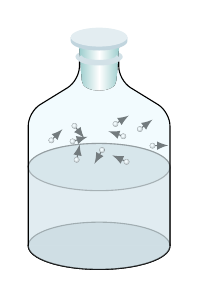
\begin{tikzpicture}[>=latex,scale=1.0]
  % \useasboundingbox(-1,-2)rectangle(8,6);
  % \draw[very thick,darkgray](0,0)--(0,1.2);
  \draw[fill=cyan!10!lightgray](0,-1.5)ellipse(0.9 and 0.3);
  \draw[fill=cyan!10!lightgray,opacity=0.5](-0.9,-0.5) arc (180:0:0.9 and 0.3)--(0.9,-1.5)arc(0:-180:0.9 and 0.3);
  \draw[fill=cyan!10!lightgray,opacity=0.5](0,-0.5) ellipse (0.9 and 0.3);
  \foreach \x/\y in {-0.607/-0.161,-0.285/-0.408,-0.337/-0.174,-0.313/ 0.023, 0.038/-0.284, 0.208/ 0.047, 0.308/-0.109, 0.349/-0.434, 0.678/-0.229, 0.518/-0.018}
  {
    \draw[->](\x,\y)--++(360*rnd:0.2);
    \fill[ball color=white](\x,\y)circle(1pt);
  }
  \draw[rounded corners=5pt,fill=cyan!10,fill opacity=0.5](-0.9,-1.5)--(-0.9,0.2)--(-0.25,0.6)--(-0.25,1.0)--(0.25,1.0)--(0.25,0.6)--(0.9,0.2)--(0.9,-1.5);
  \draw[fill=cyan!10,opacity=0.5](0.9,-1.5)arc(360:180:0.9 and 0.3);
  \fill[cyan!20!lightgray!50](0,0.9)ellipse(0.3 and 0.1);
  \fill[left color=cyan!20!lightgray,right color=cyan!20!lightgray,middle color=white](-0.22,0.6)--++(-0.04,0.5)--++(0.52,0)--++(-0.04,-0.5)to[bend left=90](-0.22,0.6)--cycle;
  \fill[cyan!20!lightgray!70](-0.36,1.1)arc(180:360:0.36 and 0.12)--++(0,0.05)--++(-0.72,0);
  \fill[cyan!20!lightgray!30](0,1.15)ellipse(0.36 and 0.12);
  \draw[cyan!20!lightgray!50,line width=2pt](-0.25,0.9)arc(180:360:0.25 and 0.075);

\end{tikzpicture}
\end{document}